
We have also examined the impact of clock drift on the ability of nodes to attain synchronicity.
According to the RBS paper, two nodes' clocks will drift apart by 1-100 micro secs. In TOSSIM,
one second is equivalent to 4 million clock ticks. Therefore, a reasonable value of node
drift lies anywhere between 4-400 ticks.  In Fig.~\ref{drift200}-~\ref{drift500}, we examine the impact
of introducing drift values within this range on a network of nodes, and how the network
is affected as more nodes initially start off with their clocks drifting apart after 1 second.
This is examined in an all-to-all topology of 10 nodes for firing function constant values 
ranging between 200-500:

\begin{figure}
\centerline{%
\includegraphics[width=6cm,angle=270]{figures/TTSvsDriftFFC200.ps}
\includegraphics[width=6cm,angle=270]{figures/GSvsDriftFFC200.ps}
}
\caption{Impact of Node Drift when FFC=200}
\label{fig:drift200}
\end{figure}


\begin{figure}
\centerline{%
\includegraphics[width=6cm,angle=270]{figures/TTSvsDriftFFC300.ps}
\includegraphics[width=6cm,angle=270]{figures/GSvsDriftFFC300.ps}
}
\caption{Impact of Node Drift when FFC=300}
\label{fig:drift300}
\end{figure}


\begin{figure}
\centerline{%
\includegraphics[width=6cm,angle=270]{figures/TTSvsDriftFFC400.ps}
\includegraphics[width=6cm,angle=270]{figures/GSvsDriftFFC400.ps}
}
\caption{Impact of Node Drift when FFC=400}
\label{fig:drift400}
\end{figure}

\begin{figure}
\centerline{%
\includegraphics[width=6cm,angle=270]{figures/TTSvsDriftFFC500.ps}
\includegraphics[width=6cm,angle=270]{figures/GSvsDriftFFC500.ps}
}
\caption{Impact of Node Drift when FFC=500}
\label{fig:drift500}
\end{figure}


\noindent
The graphs show several interesting patterns:
\begin{enumerate}\addtolength{\itemsep}{-0.5\baselineskip}
\item The error bars on the Time to Synchronize are consistently high
regardless of the number of nodes with drift and the value of the firing function constant.
\item After drift is added to at least two or three nodes, further nodes with drift
do not particularly affect the group spread in the 50th and 90th percentiles.
\item The short error bars indicate that there is very little variation in the group spread 
across different runs.
\end{enumerate}

The values of drift examined for the previous experiments ranged between 4-400 clock ticks.
The high error bars on the Time to Synchronize for these experiments, motivated us
to examine a different range of drift values. We looked at the impact of drift ranging between 
100-1000 clock ticks on 10 nodes in an all-to-all topology when the firing function constant 
is 500. Figure~\ref{fig:highdrift500} shows the results.

The observation that group spread is not particularly affected after at least two nodes in the
all-to-all topology have drift motivated us to examine the impact of the same drift values
on a grid topology. Figure~\ref{fig:drift500grid} shows the results.

\begin{figure}
\centerline{%
\includegraphics[width=6cm,angle=270]{figures/TTSvsHighDriftFFC500.ps}
\includegraphics[width=6cm,angle=270]{figures/GSvsHighDriftFFC500.ps}
}
\caption{Impact of High Node Drift (100-1000) when FFC=500}
\label{fig:highdrift500}
\end{figure}


\begin{figure}
\centerline{%
\includegraphics[width=6cm,angle=270]{figures/TTSvsDrift_GRID_FFC500.ps}
\includegraphics[width=6cm,angle=270]{figures/GSvsDrift_GRID_FFC500.ps}
}
\caption{Impact of Node Drift on a 4x4 regular grid topology when FFC=500}
\label{fig:drift500grid}
\end{figure}